\qquad Conforme orientado no enunciado do trabalho, a análise do Shell
Sort não segue o mesmo roteiro de contagem de instruções aplicado aos
demais algoritmos, pois sua complexidade depende diretamente da
sequência de intervalos (\textit{gaps}) utilizada. Em vez disso, foi
realizada uma pesquisa bibliográfica sobre a complexidade da sequência
de gaps efetivamente utilizada na implementação (a sequência original
de Shell: tamanho/2, tamanho/4, ..., 1), cujo conteúdo manuscrito é apresentado a seguir.

\begin{figure}[htbp]
    \centering
    % Substitua o arquivo abaixo pela digitalizacao da pesquisa/analise manuscrita
    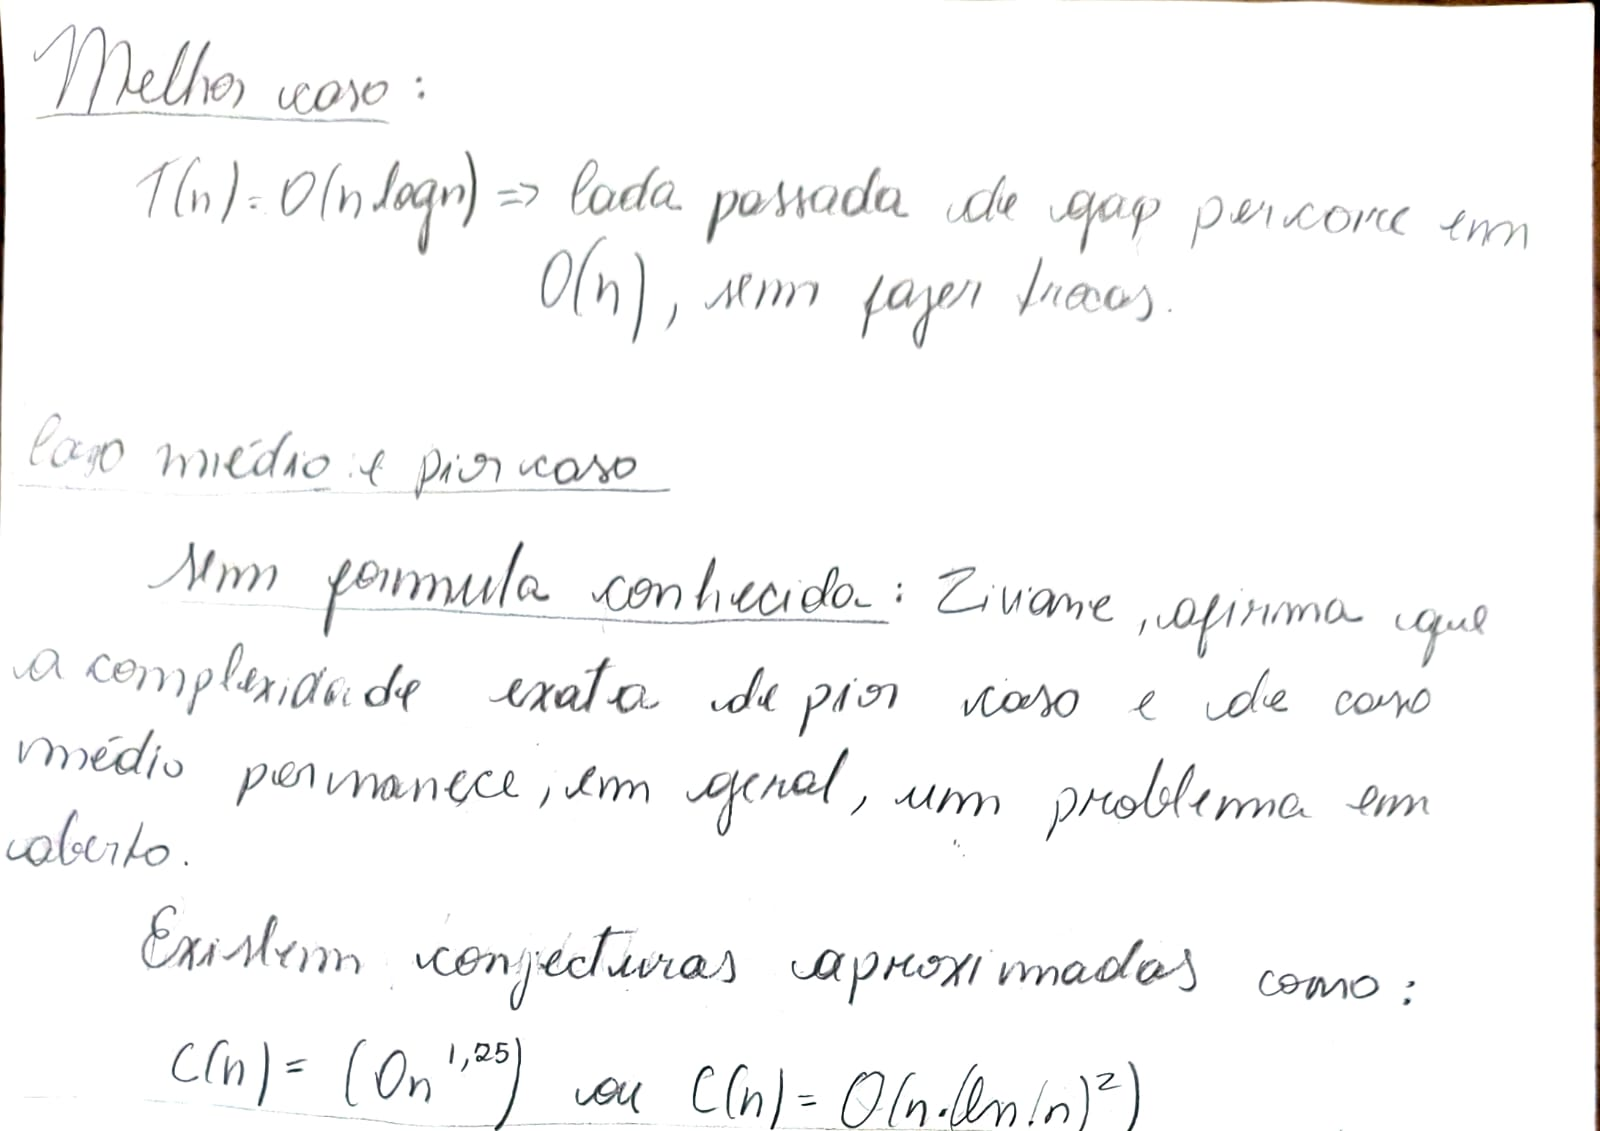
\includegraphics[width=14cm]{Imagens/Shell Sort/analise_complexidade.jpeg}
    \caption{Pesquisa e análise de complexidade manuscrita do algoritmo Shell Sort}
    \label{fig:analise_complexidade_shell}
\end{figure}

\qquad A seguir, apresenta-se essa mesma pesquisa em forma digitada,
organizada no mesmo formato de melhor/médio/pior caso adotado nos
capítulos anteriores e devidamente referenciada, para apoiar a versão
manuscrita.

\textbf{Melhor caso (entrada crescente): $T(n) = O(n \log n)$.} Cada
passada de gap percorre o vetor em $O(n)$ e, como qualquer
subsequência de um vetor já ordenado também está ordenada, nenhum
deslocamento é necessário em nenhuma passada. Como o número de
passadas é $O(\log n)$ (o gap é dividido por 2 a cada passada), o
tempo total é $T(n) = O(n \log n)$.

\textbf{Pior caso: $T(n) = \Theta(n^2)$.} Donald Knuth demonstrou que
a sequência original de Shell (potências de 2) tem pior caso
quadrático: existem entradas construídas especificamente para essa
sequência de gaps — não a simples entrada decrescente — que forçam
$\Theta(n^2)$ comparações e deslocamentos, principalmente quando $n$
é uma potência de 2 (KNUTH, 1998). É por isso que a entrada
decrescente testada neste trabalho \textbf{não} atinge esse pior
caso: qualquer subsequência de um vetor totalmente decrescente também
está em ordem decrescente, de modo que cada passada de gap continua
limitada a deslocamentos curtos, resultando em comportamento próximo
do melhor caso ($O(n \log n)$), e não do pior caso teórico.

\textbf{Caso médio (entrada randômica): sem fórmula fechada
conhecida.} Ao contrário dos três algoritmos anteriores, não existe
uma dedução simples de caso médio para o Shell Sort, e é justamente
esse ponto que justifica o caráter de pesquisa bibliográfica pedido
pelo enunciado para este capítulo. Ziviani (2012), ao apresentar o
Shellsort, afirma que a complexidade exata de pior caso e de caso
médio do algoritmo permanece, em geral, um problema em aberto: nem
mesmo para a sequência de incrementos mais estudada na literatura —
a de Knuth, $h_s = 3h_{s-1}+1$ (ou seja, $1, 4, 13, 40, 121, \ldots$),
recomendada no lugar da sequência original de Shell por ser
consideravelmente mais eficiente na prática — existe uma prova
fechada de complexidade média; há apenas \textbf{conjecturas}, como
$C(n) = O(n^{1,25})$ ou $C(n) = O(n \cdot (\ln n)^2)$ para o número de
comparações. Se até a melhor sequência de gaps conhecida tem sua
complexidade média apenas conjecturada na literatura, é esperado que
a sequência mais simples (a original de Shell, usada neste trabalho)
também não possua uma fórmula fechada de caso médio — apenas o
comportamento empírico observado nos testes, que ficou sensivelmente
abaixo de $\Theta(n^2)$ para todos os tamanhos testados.

\qquad Em resumo, a escolha da sequência de gaps é o fator decisivo na
complexidade do Shell Sort — um ponto reforçado tanto por Knuth
(1998), que provou o pior caso quadrático da sequência original, quanto
por Ziviani (2012), que recomenda sequências mais sofisticadas
justamente por essa sensibilidade à sequência escolhida. Ainda assim,
mesmo utilizando a sequência mais simples possível, o Shell Sort
superou folgadamente Insertion, Selection e Bubble Sort na prática,
para todos os tipos de entrada testados neste trabalho, como mostram os resultados da próxima seção; a comparação com o Merge Sort é feita na Tabela de Comparação e na Conclusão.
